In questo capitolo parleremo delle tecnologie usate per la realizzazione del progetto X-Project.
Le tecnologie usate nel lato server sono MongoDB, NodeJS e LoopBack di StrongLoop. MongoDB è un DBMS non relazionale, orientato ai documenti; NodeJS è un framework event-driven relativo all'utilizzo server-side di Javascript mentre LoopBack è un framework realizzato da un insieme di moduli NodeJS con lo scopo di realizzare in modo veloce e semplice API per uso di applicazioni generali.
Per il lato client abbiamo usato HTML5 un linguaggio di markup per la struttutazione delle pagine web, Polymer che è un'estensione open-source di Web Components e questo framework sta alla base dell'interfaccia utente di Android L e delle nuove regole del Material Design in grado di funzionare su tutti i fattori di forma, tutti i dispositivi e piattaforme.


\begin {figure}[h]
\graphicspath{{images/chapter_TCH/}}
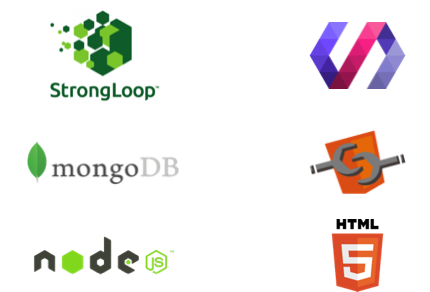
\includegraphics[width=\textwidth]{stack_tch}
\end {figure}


In this chapter.